
% \jb{ToDo: less emphasize theoretical results -- I think our current flow is not that problematic, but anyway we need to follow the reivew a little bit at least...}
% \kj{What about change the section title? something like Relationship between Flat Minima and Domain Generalization Gap}

Let $\mathcal{D}:=\left\{\mathcal{D}_{i}\right\}_{i}^{I}$ be a set of training domains, where $\mathcal{D}_{i}$ is a distribution over input space $\mathcal{X}$, and $I$ is the total number of domains. From each domain, we observe $n$ training data points which consist of input $x$ and target label $y$, $(x_{j}^{i},y_{j}^{i})_{j=1}^{n}\sim\mathcal{D}_{i}$.
We also define a set of target domain $\mathcal{T}:=\left\{\mathcal{T}_{i}\right\}_{i}^{T}$ similarly, where the number of target domains $T$ is usually set to one.
For the sake of simplicity, unlike \citet{ben2010theory},
we assume that there exists a global labeling function $h(x)$ that generates target label for multiple domains, \ie, $y_{j}^{i}=h(x_{j}^{i})$ for all $i$ and $j$.
Domain generalization (DG) aims to find a model parameter $\theta \in \Theta$ which generalizes well over both multiple training domains $\mathcal{D}$ and unseen target domain $\mathcal{T}$.
More specifically, let us consider a bounded instance loss function $\ell:\mathcal{Y}\times\mathcal{Y} \rightarrow [0, c]$,
% \footnote{While we assume that $\ell(\cdot,\cdot)$ is bounded by one, it can be generalized for any bounded loss function.}
such that $\ell(y_{1},y_{2})=0$ holds if and only if $y_{1}=y_{2}$ where $\mathcal{Y}$ is a set of labels.
For simplicity, we set $c$ to one in our proofs, but we note that $\ell(\cdot,\cdot)$ can be generalized for any bounded loss function.
Then, we can define a population loss over multiple domains by $\mathcal{E}_{\mathcal{D}}(\theta)=\frac{1}{I}\sum_{i=1}^{I}\mathbb{E}_{x^{i}\sim\mathcal{D}_{i}}[\ell(f(x^{i};\theta), y^{i}))]$, where $f(\cdot;\theta)$ is a model parameterized by $\theta$.
Formally, the goal of DG is to find a model which minimizes both $\mathcal{E}_{\mathcal{D}}(\theta)$ and $\mathcal{E}_{\mathcal{T}}(\theta)$ by only minimizing an empirical risk $\hat{\mathcal{E}}_{\mathcal{D}}(\theta):=\frac{1}{In}\sum_{i=1}^{I}\sum_{j=1}^{n}\ell(f(x^{i};\theta), y^{i}))$ over training domains $\mathcal D$.

%In practice, ERM, \ie, $\arg\min_\theta \hat{\mathcal{E}}_{\mathcal{D}}(\theta)$, is non-convex and has multiple local minima whose solution parameters are similar in terms of the training loss $\hat{\mathcal{E}}_{\mathcal{D}}(\theta)$, but significantly different in terms of the generalization performances $\mathcal{E}_{\mathcal{D}}(\theta)$ and $\mathcal{E}_{\mathcal{T}}(\theta)$.
In practice, ERM, \ie, $\arg\min_\theta \hat{\mathcal{E}}_{\mathcal{D}}(\theta)$, can have multiple solutions that provide similar values of the training losses but significantly different generalizability on $\mathcal{E}_{\mathcal{D}}(\theta)$ and $\mathcal{E}_{\mathcal{T}}(\theta)$.
% In practice, $\arg\min_\theta \hat{\mathcal{E}}_{\mathcal{D}}(\theta)$ is a non-convex problem and has multiple local minimum which have similar training loss, $\hat{\mathcal{E}}_{\mathcal{D}}(\theta)$, but whose true loss ar significantly different in terms of the generalization performances, $\mathcal{E}_{\mathcal{D}}(\theta)$ and $\mathcal{E}_{\mathcal{T}}(\theta)$.
Unfortunately, the typical optimization methods, such as SGD and Adam~\cite{kingma2015adam}, often lead sub-optimal generalizability as finding sharp and narrow minima even under the i.i.d. assumption~\cite{keskar2016largebatch,dziugaite2017computing,garipov2018fge,izmailov2018swa,jiang2019fantastic,foret2020sharpness}.
In the DG scenario, the generalization gap between empirical loss and target domain loss becomes even worse
% than i.i.d. assumption 
due to domain shift.
Here, we provide a theoretical interpretation of the relationship between finding a flat minimum and minimizing the domain generalization gap, inspired by previous studies~\cite{keskar2016largebatch,dziugaite2017computing,garipov2018fge,izmailov2018swa,jiang2019fantastic,foret2020sharpness}.

\begin{wrapfigure}{r}{0.41\linewidth}
    \centering
%    \vspace{-1em}
    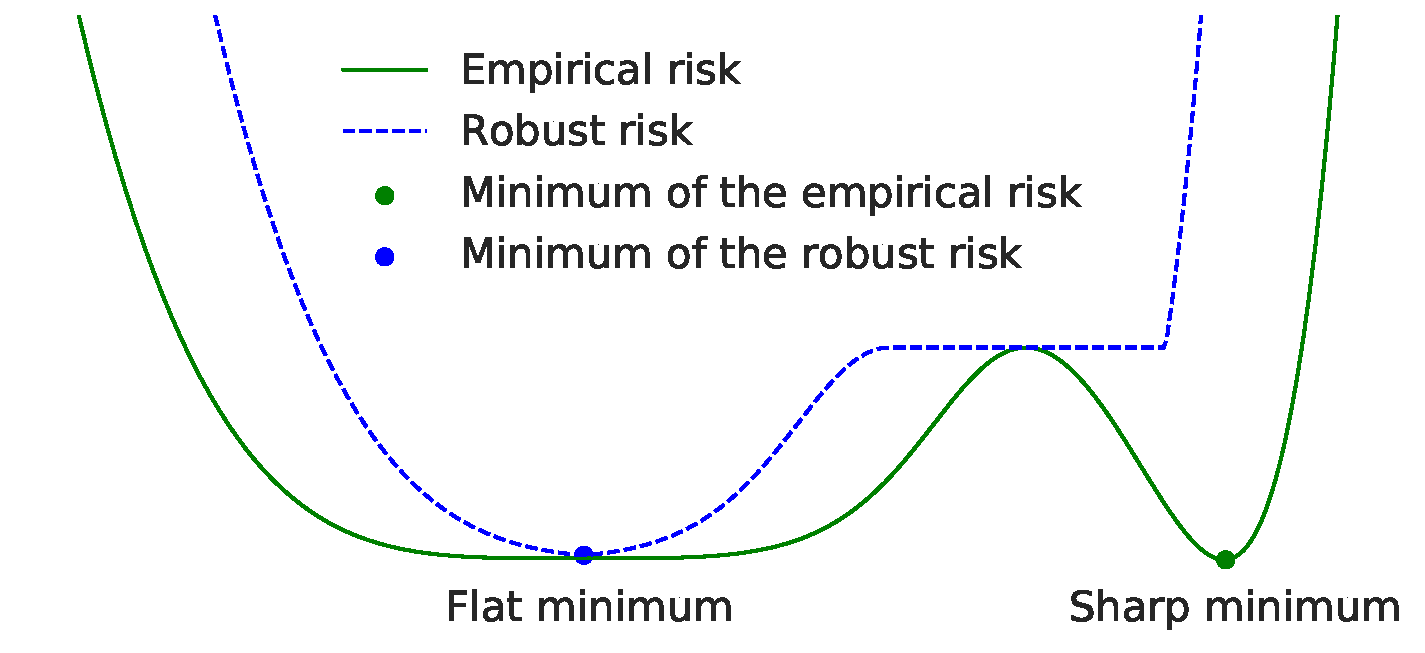
\includegraphics[width=\linewidth]{figures/rrm_concept_fig.pdf}
    \caption{\small {\bf Robust risk minimization (RRM) and flat minima.} With proper $\gamma$, RRM will find flat minima.}
    \label{fig:rrm_and_flatoptima}
    \vspace{-1.8em}
\end{wrapfigure}
We consider a robust empirical loss function defined by the worst-case loss within neighborhoods in the parameter space as $\hat{\mathcal{E}}_{\mathcal{D}}^{\gamma}(\theta):=\max_{\|\Delta\|\leq\gamma} \hat{\mathcal{E}}_{\mathcal{D}}(\theta+\Delta)$, where $\|\cdot\|$ denotes the L2 norm and $\gamma$ is a radius which defines neighborhoods of $\theta$.
Intuitively, if $\gamma$ is sufficiently larger than the ``radius'' of a sharp optimum $\theta_s$ of $\hat{\mathcal{E}}_{\mathcal{D}}(\theta)$, $\theta_s$ is no longer an optimum of $\hat{\mathcal{E}}_{\mathcal{D}}^{\gamma}(\theta)$ as well as its neighborhoods within the $\gamma$-ball.
On the other hand, if an optimum $\theta_f$ has larger ``radius'' than $\gamma$, there exists a local optimum within $\gamma$-ball -- See Figure~\ref{fig:rrm_and_flatoptima}.
Hence, solving the robust risk minimization (RRM), \ie, $\arg\min_\theta \hat{\mathcal{E}}_{\mathcal{D}}^{\gamma}(\theta)$, will find a near solution of a flat optimum showing better generalizability~\cite{norton2019diametrical, foret2020sharpness}.
However, as domain shift worsen the generalization gap by breaking the i.i.d. assumption, it is not trivial that RRM will find an optimum with better DG performance.
% as the i.i.d. scenario.
To answer the question,
% we provide a theorem, showing that finding a flat minimum by RRM, $\hat{\mathcal{E}}_{\mathcal{D}}^{\gamma}(\theta)$, bounds the loss for the unseen target domain $\mathcal T$, $\mathcal{E}_{\mathcal{T}}(\theta)$ (Theorem~\ref{thm:gen_bnd_dg_final}).
we first show the generalization bound between $\hat{\mathcal{E}}^{\gamma}_{\mathcal{D}}$ and $\mathcal{E}_{\mathcal{T}}$ as follows:
\begin{theorem}\label{thm:gen_bnd_dg}
Consider a set of $N$ covers $\{\Theta_{k}\}_{k=1}^{N}$ such that the parameter space $\Theta \subset \cup_{k}^{N} \Theta_{k}$ where $diam(\Theta):=\sup_{\theta,\theta'\in \Theta}\|\theta-\theta'\|_{2}$, $N:=\left\lceil\left(diam(\Theta)/\gamma\right)^{d}\right\rceil$ and $d$ is dimension of $\Theta$.
Let $v_{k}$ be a VC dimension of each $\Theta_{k}$.
Then, for any $\theta\in\Theta$, the following bound holds with probability at least $1-\delta$,
\begin{equation}
\label{eq:thm1_bound}
\mathcal{E}_{\mathcal{T}}(\theta) < \hat{\mathcal{E}}_{\mathcal{D}}^{\gamma}(\theta) +\frac{1}{2I}\sum_{i=1}^{I}\mathbf{Div}(\mathcal{D}_{i},\mathcal{T})+ \max_{k\in[1,N]} \sqrt{\frac{v_{k}\ln\left(m/v_{k}\right)+\ln(N/\delta)}{m}},
\end{equation}
where $m = nI$ is the number of the training samples and $\mathbf{Div}(\mathcal{D}_{i},\mathcal{T}):=2\sup_{A}|\mathbb{P}_{\mathcal{D}_{i}}(A)-\mathbb{P}_{\mathcal{T}}(A)|$ is a divergence between two distributions.
\end{theorem}
Proof can be done similarly as \cite{ben2010theory} and \cite{norton2019diametrical}.
% \kj{Note that proof can be done by using the similar techniques in \cite{ben2010theory} and \cite{norton2019diametrical}.}
In Theorem~\ref{thm:gen_bnd_dg}, the test loss $\mathcal{E}_{\mathcal{T}}(\theta)$ is bounded by three terms: (1) the robust empirical loss $\hat{\mathcal{E}}_{\mathcal{D}}^{\gamma}(\theta)$, (2) the discrepancy between training distribution and test distribution, \ie, the quantity of domain shift, and (3) a confidence bound related to the radius $\gamma$ and the number of the training samples $m$.
Our theorem is similar to \citet{ben2010theory}, while our theorem does not have the term related to the difference in labeling functions across the domains. It is because we simply assume there is no difference between labeling functions for each domain for simplicity. If one assumes a different labeling function, the dissimilarity term can be derived easily because it is independent and compatible with our main proof.
More details of Theorem~\ref{thm:gen_bnd_dg}, including proof and discussions on the confidence bound, are in Appendix C.1 and C.2.
% Here, since increasing $\gamma$ decreases $N$, \ie, grows $|\Theta_k|$, $v_k$, the VC dimension of each cover $\Theta_k$ is increased.
% Note that the relationship between $\gamma$ and the confidence bound is the same as that of \citet{foret2020sharpness}.

From Theorem~\ref{thm:gen_bnd_dg}, one can conjure that minimizing the robust empirical loss is directly related to the generalization performances on the target distribution.
We show that the domain generalization gap on the target domain $\mathcal T$ by the optimal solution of RRM, $\hat{\theta}^{\gamma}$, is upper bounded as follows:
\begin{theorem}\label{thm:gen_bnd_dg_final}
Let $\hat{\theta}^{\gamma}$ denote the optimal solution of the RRM, \ie, $\hat{\theta}^{\gamma}:=\arg\min_{\theta}\hat{\mathcal{E}}^{\gamma}_{\mathcal{D}}(\theta)$, and let $v$ be a VC dimension of the parameter space $\Theta$.
Then, the gap between the optimal test loss, $\min_{\theta'}\mathcal{E}_{\mathcal{T}}\left(\theta'\right)$, and the test loss of $\hat{\theta}^{\gamma}$, $\mathcal{E}_{\mathcal{T}}(\hat{\theta}^{\gamma})$, has the following bound with probability at least $1-\delta$.
\begin{align}
\begin{split}
    \mathcal{E}_{\mathcal{T}}(\hat{\theta}^{\gamma}) - \min_{\theta'}\mathcal{E}_{\mathcal{T}}&\left(\theta'\right) \quad \leq \quad \hat{\mathcal{E}}_{\mathcal{D}}^{\gamma}(\hat{\theta}^{\gamma}) - \min_{\theta''}\hat{\mathcal{E}}_{\mathcal{D}}(\theta'') + \frac{1}{I}\sum_{i=1}^{I}\mathbf{Div}(\mathcal{D}_{i},\mathcal{T})\\
    &+ \max_{k\in[1,N]} \sqrt{\frac{v_{k}\ln\left(m/v_{k}\right)+\ln\left(2N/\delta\right)}{m}} + \sqrt{\frac{v\ln\left(m/v\right) + \ln\left(2/\delta\right)}{m}}
\end{split}
\end{align}
\end{theorem}
Proof is in Appendix C.3. It implies that if we find the optimal solution of the RRM (\ie, $\hat{\theta}^{\gamma}$), then the generalization gap in the test domain (\ie, $\mathcal{E}_{\mathcal{T}}(\hat{\theta}^{\gamma}) - \min_{\theta'}\mathcal{E}_{\mathcal{T}}\left(\theta'\right)$) is upper bounded by the gap between the RRM and ERM (\ie,
$\hat{\mathcal{E}}_{\mathcal{D}}^{\gamma}(\hat{\theta}^{\gamma}) - \min_{\theta''}\hat{\mathcal{E}}_{\mathcal{D}}(\theta'')$).
Other terms in Theorem~\ref{thm:gen_bnd_dg_final} are the discrepancy between the train domains $\mathcal D$ and the target domain $\mathcal T$, and the confidence bounds caused by sample means.
We remark that if we choose a proper $\gamma$, the optimal solution of the RRM will find a point near a flat optimum of ERM as shown in Figure~\ref{fig:rrm_and_flatoptima}.
Hence, Theorem~\ref{thm:gen_bnd_dg_final} and the intuition from Figure~\ref{fig:rrm_and_flatoptima} imply that seeking a flat minimum of ERM will lead to a better domain generalization gap.
% Hence, if we can find a flat minimum of ERM near $\hat{\theta}^{\gamma}$, then it will show better generalizability than $\hat{\theta}^{\gamma}$ because the right-hand side in Theorem~\ref{thm:gen_bnd_dg_final} can be reduced.
% More discussions related to Theorem~\ref{thm:gen_bnd_dg_final} are in \S\ref{s_discussion} and Appendix.
% Furthermore, obviously, collecting more training data also increases generalization performance at test time by reducing the confidence error bounds which are the third and final term. 
% The second term cannot be controlled since domain generalization assumes that we cannot use any clue for test distribution in training phase.
% {\bf While the last term tells effect of $\gamma$ on generalization error bound, there exists a limitation in that the last term cannot represent the behavior of confidence bound with respect to $\gamma$ since the bound diverges to infinity when $\gamma$ goes to zero. However, we would like to note that this limitation is not a drawback of RRM, but it is caused by looseness of union bound which is a mathematical technique used to derive the last term.}


\iffalse

\sh{Missings -- Div discussions related to the loss surface figure. Where can we add it? Clean up notations and abbreviation (RRM)}

\sh{TODO -- Appendix: proofs, discussions on theoretical bounds}

\kj{UPDATE:
Consider an instance loss function $l(y_{1}, y_{2})$
such that $l:\mathcal{Y}\times\mathcal{Y} \rightarrow [0, M]$ and $l(y_{1},y_{2})=0$ iff $y_{1}=y_{2}$.
Then, we can define a functional error as $\mathcal{E}_{\mathcal{P}}(f(\cdot;\theta),h):=\mathbb{E}_{\mathcal{P}}[l(f(x;\theta),h(x))]$.
Note that if we set $h$ as a true label function which generates the label of inputs, $y=h(x)$,
then, it becomes a population loss $\mathcal{E}_{\mathcal{P}}(\theta)=\mathcal{E}_{\mathcal{P}}(f(\cdot;\theta),h)$.
\begin{lemma}
$\left|\mathcal{E}_{\mathcal{P}}(h_{1},h_{2}) - \mathcal{E}_{\mathcal{Q}}(h_{1},h_{2})\right| \leq \frac{M}{2}\mathbf{Div}(\mathcal{P},\mathcal{Q})$
\end{lemma}
\begin{proof}
From the Fubini's theorem, we have,
\begin{align}
    \mathbb{E}_{x\sim\mathcal{P}}[l(h_{1}(x),h_{2}(x))] = \int_{0}^{\infty} \mathbb{P}_{\mathcal{P}}\left(l(h_{1}(x),h_{2}(x)) > t\right) dt
\end{align}
By using this fact, 
\begin{align}
    &\left|\mathbb{E}_{x\sim\mathcal{P}}[l(h_{1}(x),h_{2}(x))]- \mathbb{E}_{x\sim\mathcal{Q}}[l(h_{1}(x),h_{2}(x))]\right|\\
    &= \left|\int_{0}^{\infty} \mathbb{P}_{\mathcal{P}}\left(l(h_{1}(x),h_{2}(x)) > t\right) dt - \int_{0}^{\infty} \mathbb{P}_{\mathcal{Q}}\left(l(h_{1}(x),h_{2}(x)) > t\right) dt\right|\\
    &\leq \int_{0}^{\infty} \left|\mathbb{P}_{\mathcal{P}}\left(l(h_{1}(x),h_{2}(x)) > t\right) -  \mathbb{P}_{\mathcal{Q}}\left(l(h_{1}(x),h_{2}(x)) > t\right) \right|dt\\
    &\leq M\sup_{t\in[0,M]} \left|\mathbb{P}_{\mathcal{P}}\left(l(h_{1}(x),h_{2}(x)) > t\right) -  \mathbb{P}_{\mathcal{Q}}\left(l(h_{1}(x),h_{2}(x)) > t\right) \right|\\
    &\leq M\sup_{h_{1},h_{2}}\sup_{t\in[0,M]} \left|\mathbb{P}_{\mathcal{P}}\left(l(h_{1}(x),h_{2}(x)) > t\right) -  \mathbb{P}_{\mathcal{Q}}\left(l(h_{1}(x),h_{2}(x)) > t\right) \right|\\
    &\leq M\sup_{\bar{h}\in\bar{\mathcal{H}}}\left|\mathbb{P}_{\mathcal{P}}\left(\bar{h}(x)=1\right) -  \mathbb{P}_{\mathcal{Q}}\left(\bar{h}(x)=1\right) \right|\\
    &\leq M\sup_{A}\left|\mathbb{P}_{\mathcal{P}}\left(A\right) -  \mathbb{P}_{\mathcal{Q}}\left(A\right) \right|
\end{align}
where $\bar{\mathcal{H}}:=\left\{\mathbb{I}[l(h(x),h'(x))>t]\middle|h,h'\in\mathcal{H}, t \in [0,M]\right\}$.
\end{proof}
\begin{itemize}
    \item Why do we need boundness of loss function? 
    \begin{itemize}
        \item 1. In order to make the integral bounded.
        \item 2. In order to use the Hoeffding inequality.
    \end{itemize}
    \item Pros: Now, we can cover more general loss function.
    \item Cons: But it should be bounded, which cannot cover cross entropy...
\end{itemize}
}
\fi